% Chapter Template
\chapter{!!NOT DONE!! Computational Setup, !!NOT DONE!!} % Main chapter title

\label{Chapter4} % Change X to a consecutive number; for referencing this chapter elsewhere, use \ref{ChapterX}


\section{Introduction}

%----------------------------------------------------------------------------------------
%	SECTION 1
%----------------------------------------------------------------------------------------
\section{Monte Carlo event Generation}
\subsection{Heavy Neutrino signal event Generation}
\subsection{SM background event Generation}
\subsection{Benchmark Heavy Neutrino Inputs}

\section{Signal simulation}
\label{sec:signal}
%{\bf (Tom)}\vspace*{2ex}\\

Signal samples are generated using the \MGvATNLO
generator~\cite{Alwall:2014hca} at leading order (LO) in the strong
coupling constant $\alpha_{\mathrm{S}}$.
The generation is based on the \texttt{heavyN} model described in
Ref.~\cite{Atre:2009rg}, which is availabe in Universal FeynRules
Output (UFO) by Ref.~\cite{Alva:2014gxa,Degrande:2016aje}.
The UFO files for the \texttt{heavyN} model are found at
Ref.~\cite{heavyN}.
This model extends the SM with up to three right-handed neutrinos,
which are singlets under the SM gauge symmetry.
The mass and mixing parameters of the HNL can be defined by the user.
The width $\Gamma_{\hnl}$ is computed automatically by the
generator, and the mean lifetime $\tau_{\hnl} = \hbar/\Gamma_{\hnl}$
is used to extract the HNL lifetime in each simulated event,
according to a decay probability distribution
$dN(t)/dt = \frac{1}{\tau_{\hnl}}e^{-t/\tau_{\hnl}}$, where $t$ is the
\emph{proper} lifetime, measured in the HNL rest frame.

For our signal simulation, we consider HNLs of masses
$\mhnl = 1$--$20\GeV$, which couple
exclusively to one of the three SM neutrino families with different
mixing probabilities, typically in a range $10^{-5}$--$10^{-2}$,
depending on the mass:
\begin{linenomath}
\begin{equation}
  \mathbf{V}_{\hnl\ell} =
  \begin{pmatrix}
    \mathrm{V}_{\hnl\Pe} & 0 & 0 \\
    0                   & 0 & 0 \\
    0                   & 0 & 0 \\
  \end{pmatrix},
%% \end{equation}
\quad\quad
%% \begin{equation}
  \mathbf{V}_{\hnl\ell} =
  \begin{pmatrix}
    0                    & 0 & 0 \\
    \mathrm{V}_{\hnl\PGm} & 0 & 0 \\
    0                    & 0 & 0 \\
  \end{pmatrix},
%% \end{equation}
\quad\quad
%% \begin{equation}
  \mathbf{V}_{\hnl\ell} = 
  \begin{pmatrix}
    0                    & 0 & 0 \\
    0                    & 0 & 0 \\
    \mathrm{V}_{\hnl\PGt} & 0 & 0 \\
  \end{pmatrix},
\end{equation}
\end{linenomath}
where $\mathbf{V}_{\hnl\ell}$ represents the active-sterile neutrino
mixing matrix:
\begin{linenomath}
\begin{equation}
  \begin{pmatrix}
    \nu_{\Pe}  \\
    \nu_{\PGm} \\
    \nu_{\PGt} \\
  \end{pmatrix} ~=~
  \mathbf{V}_{\hnl\ell}\,\cdot\,
  \begin{pmatrix}
    \hnl_{1} \\
    \hnl_{2} \\
    \hnl_{3} \\
  \end{pmatrix}.
\end{equation}
\end{linenomath}

As explained in Section~\ref{sec:promptll}, the values of \mhnl
and \mixpar do not only determine the HNL production cross section,
but also its mean lifetime and, consequently, its kinematics,
acceptance, and reconstruction efficiency.
For a fixed value of \mhnl, therefore, a simple cross section
rescaling is not sufficient to correctly reproduce the behavior of
other HNLs with same mass and different \mixpar.
To this purpose, we use instead a per-event re-weighting technique
based on the HNL lifetime, which properly accounts for all the
variations in kinematics and acceptance.
First, we notice that the average kinematics of a HNL decay
%in a given event
is entirely defined by the HNL mass \mhnl, its momentum
$p_\hnl=\beta\gamma\mhnl$, and its decay length,
%(or, equivalently, its decay time $t_\hnl$),
independently of its mean lifetime $\tau_\hnl$.
Therefore, given a simulated HNL sample of mass \mhnl and mean
lifetime $\tau_0$, we can reproduce the kinematic distributions of any
other HNL with same mass and different mean lifetime $\tau_1$ by
simply re-weighting each event---with proper decay time
$t$---by the ratio of probabilities to obtain a lifetime of $t$ for
mean lifetimes $\tau_0$ and $\tau_1$: 
\begin{linenomath}
  \begin{equation}
    W(t) ~=~ \frac{dN_1(t)/dt}{dN_0(t)/dt} ~=~
    \frac{\tau_0}{\tau_1}\exp{\left[-t\left(\frac{1}{\tau_1}-\frac{1}{\tau_0}\right)\right]}.
  \end{equation}
  \label{eq:ctauReweighting}
\end{linenomath}
Note that
$\tau_0/\tau_1 = |\mathrm{V_{\hnl\ell,1}}|^2/|\mathrm{V_{\hnl\ell,0}}|^2$,
therefore this method allows us to move along the \mixpar axis of the
$(\mhnl,\mixpar)$ plane.


\section{Dirac HNL signal emulation}
\label{sec:signalDirac}
The HNL production cross section is fixed by the \mhnl and \mixpar
values~\cite{Degrande:2016aje,heavyN}, and is the same for Dirac and
Majorana HNLs.
The resonance width for a Majorana HNL, on the other hand, is exactly
twice the width of a Dirac HNL with same \mhnl--\mixpar values, due to
the additional charge-conjugated (LNV) decay channels.
As a consequence, the average lifetime of a Dirac HNL is twice that of
a Majorana HNL with same $(\mhnl,\mixpar)$.

To optimize computing resources and in the interest of time,
high-statistics MC samples were produced on a large scale for Majorana
HNL scenarios only, both privately by the analysis authors and via the
central CMS MC production system.
Dirac HNL scenarios for any $(\mhnl,\mixpar)$ point were emulated
starting from the corresponding Majorana HNL samples, following these
steps:
\begin{itemize}
\item from a Majorana HNL sample, select only the LNC events by
  looking at the PDG ID of the generated particles;
\item reweight each LNC event to emulate the correct lifetime of the
  Dirac HNL, by using Eq.~\ref{eq:ctauReweighting} with
  $\tau_1=2\tau_0$;
\item since only half the events of the original Majorana sample are
  used (while the cross section is the same for Majorana and Dirac
  scenarios), add a factor 2 to the event weight to restore the correct
  normalization.
\end{itemize}
This method provides a good modeling of the Dirac HNL signal, but
uses only half the events from the Majorana HNL MC samples. With a
simple extra assumption, it is possible to make use of the full
statistical power of our MC production.

As explained in the following sections, the signal selection is the
same for LNC and LNV events. Just in the final stage of the analysis,
events are split into same-lepton-charge and opposite-lepton-charge
categories to distinguish LNV and LNC events for the physics
interpretation. If we assume that the lepton efficiency and
acceptance are the same for positively and negatively charged leptons
(\ie, same reconstruction and identification efficiency, same momentum
scale and resolution, etc.), then we can use both LNC and LNV events
from the Majorana HNL samples to emulate the Dirac scenarios, and
simply classify all of them as opposite-charge events. In fact, any
difference in the performance of positive and negative leptons is
expected to be negligible, certainly well below the systematic
uncertainties assigned to the displaced leptons (see
Section~\ref{sec:nonpromptleptoneffsysts}).
This approach allows us to use all the available events from the
Majorana HNL samples in the Dirac HNL interpretation.

Figure~\ref{fig:majToDirReweighting} shows a comparison between Dirac
HNL samples and Majorana HNL samples corrected to emulate Dirac
scenarios, employing both strategies outlined above.
%(\ie, using only LNC events or all events).
As can be seen, differences are small in all bins.
\begin{figure}[h!]
  \centering
  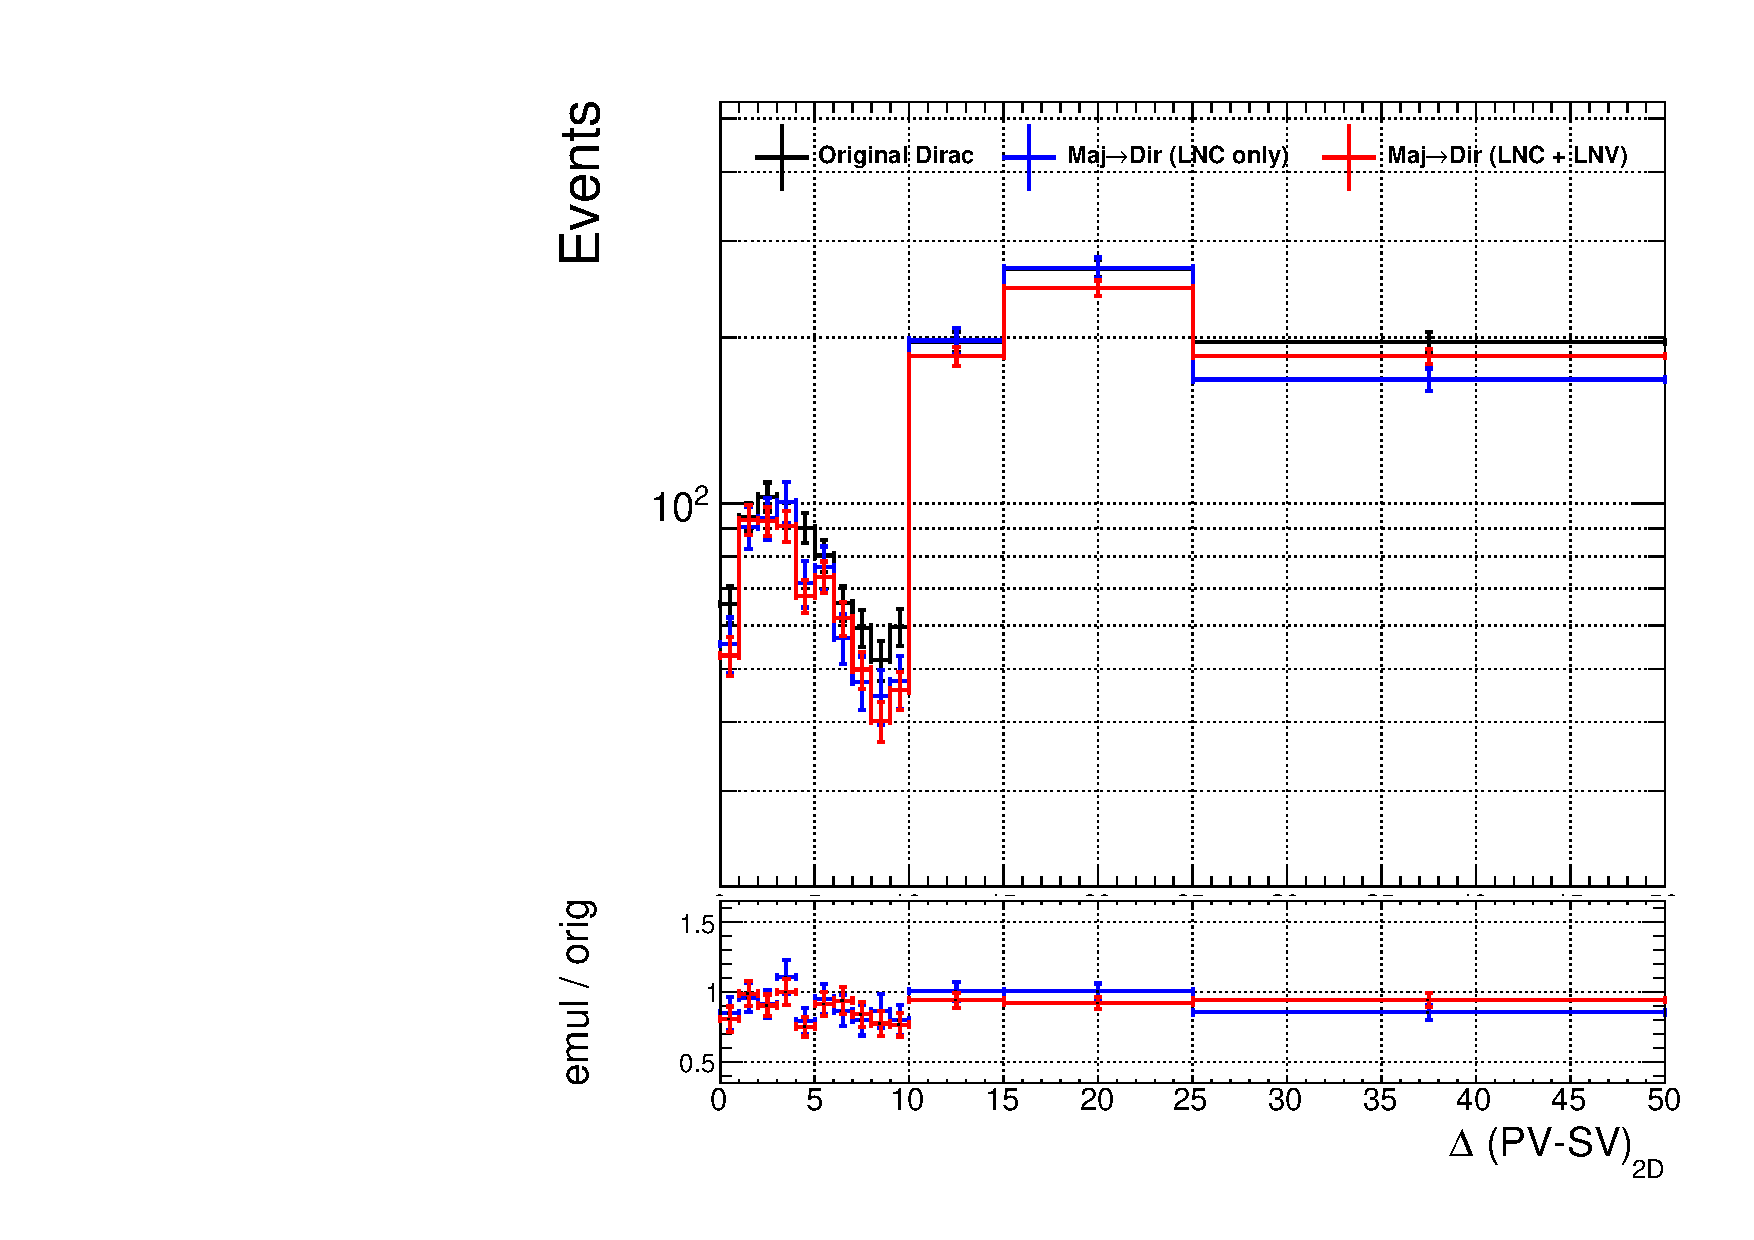
\includegraphics[width = .58\textwidth]{Figures/c4/M-3_V-0p0140356688476_mu_Dirac_from_Majorana_mu_DeltaPV_SV_2D__0.pdf}\\
  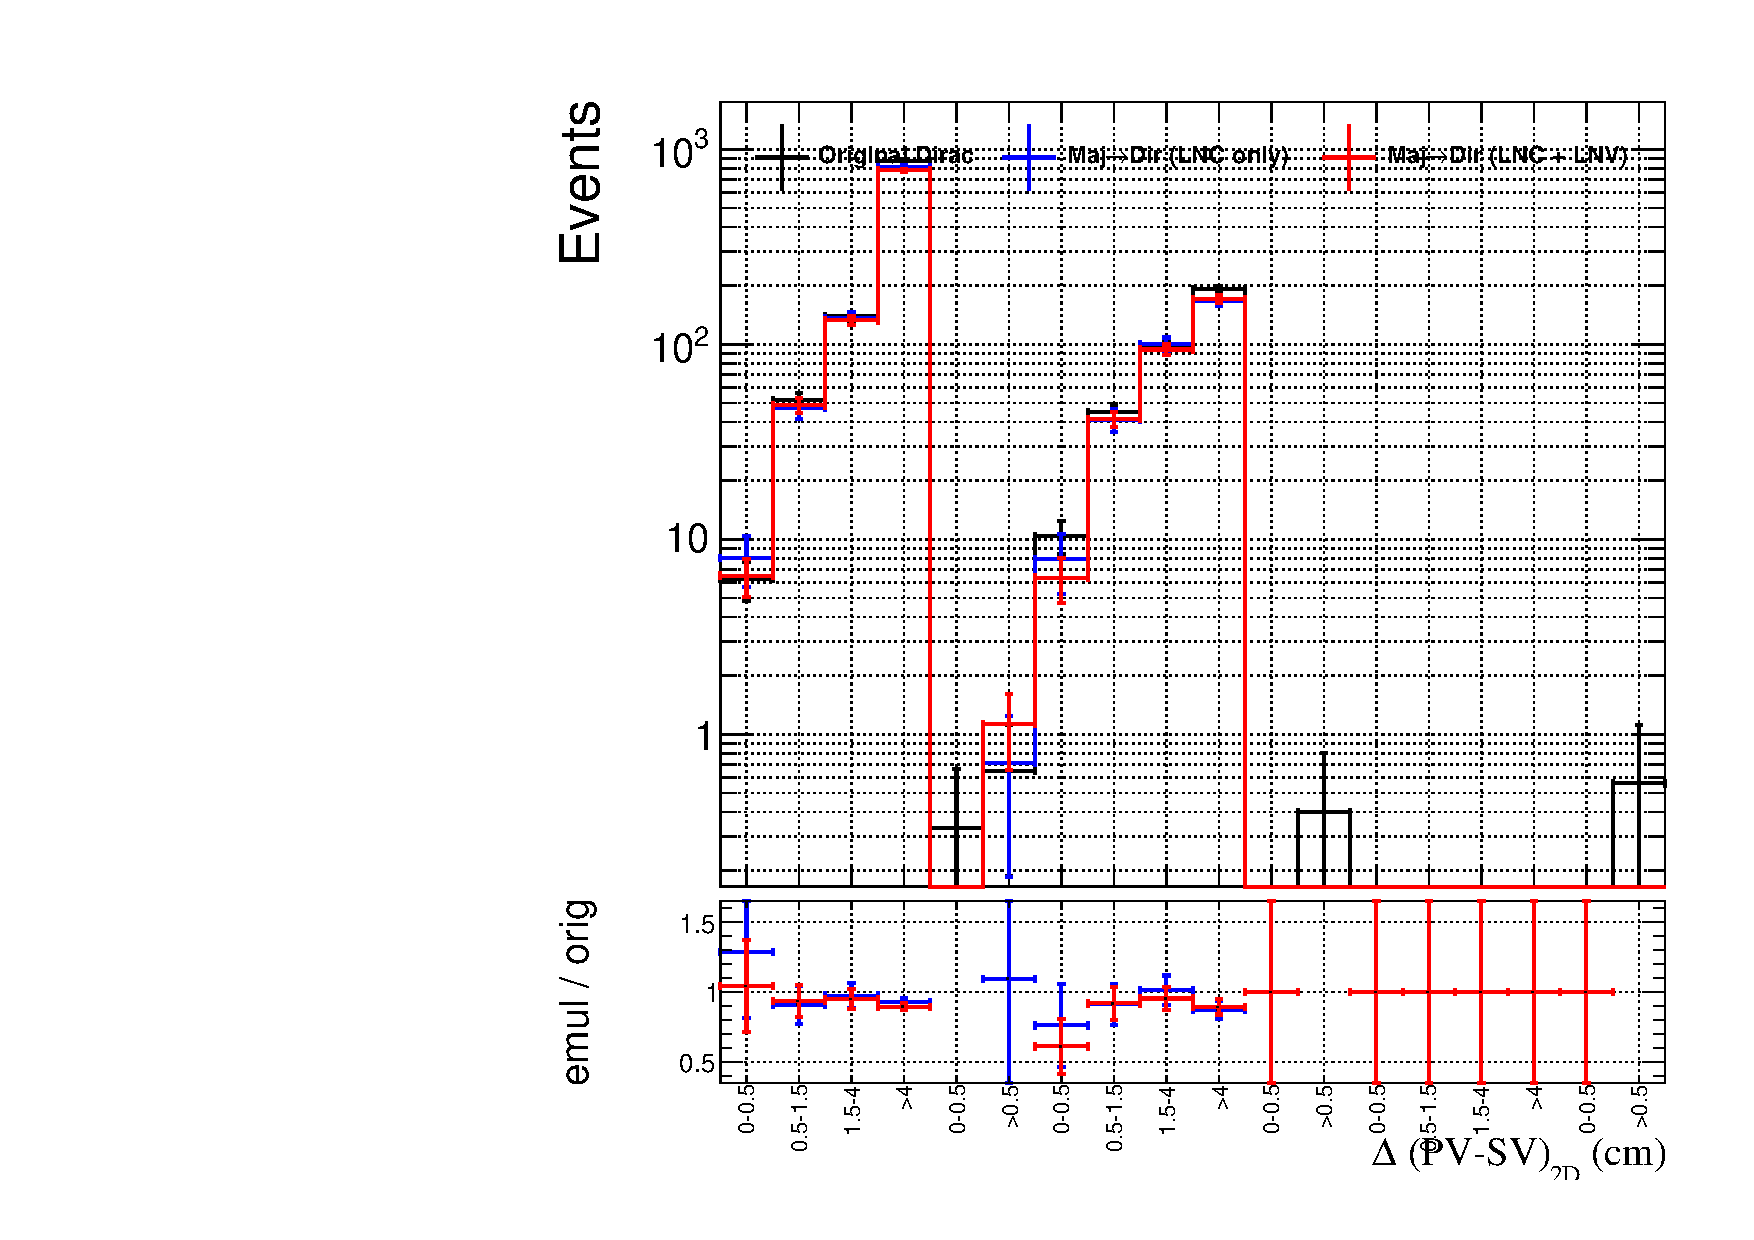
\includegraphics[width = .58\textwidth]{Figures/c4/M-3_V-0p0140356688476_mu_Dirac_from_Majorana_mu_SR__0.pdf}
  \caption{Transverse displacement of the reconstructed HNL decay
    vertex \Deltwod (top) and event yields in the different analysis
    categories described in Section~\ref{sec:baselinesel} (bottom)
    for a Dirac HNL with $\mhnl=3\GeV$
    and $\mixparm=2\times 10^{-4}$, using three models:
    a Dirac HNL sample (black), or a Majorana HNL sample with
    $\mhnl=3\GeV$ and $\mixparm=10^{-4}$, reweighted to emulate the
    Dirac scenario with $\mixparm=2\times 10^{-4}$, using LNC events
    only (blue) or all events (red).}
  \label{fig:majToDirReweighting}
\end{figure}

\section{Trigger, data sets and simulated samples}
\label{sec:dataset}
%{\bf (Riccardo, Vinzenz, DeHua)}\vspace*{2ex}\\

The current analysis uses three sets of $\Pp\Pp$ collision data at a
center-of-mass energy of 13\TeV, corresponding to integrated
luminosities of 35.92\fbinv (2016), 41.53\fbinv (2017), and 59.97\fbinv
(2018). Several primary data sets (PD) are used to search for HNLs decaying
to different lepton flavors, as well as to build control regions for
background estimation:
\begin{itemize}
\item SingleElectron (EGamma in 2018);
\item SingleMuon;
\item DoubleEG (EGamma in 2018);
\item DoubleMuon.
%\item MuonEG.
\end{itemize}
Possible overlaps among different data sets are
removed by checking run, lumi-section, and event numbers in order to not have twice the same event coming from different PDs.

Every HNL signal event contains one prompt lepton and two (generally)
\displ leptons. Since (most of) the CMS leptonic triggers are
optimized for prompt lepton identification,
we opt for the use of single-electron and single-muon triggers for the
signal selection, as listed in Table~\ref{tab:sgnlTriggers}.
The trigger efficiency in  Monte Carlo (MC) samples is corrected
according to the efficiency observed in data, by using per-event scale
factors (SFs) as a function of the prompt lepton \pt and $\eta$.
In order to make this correction possible, the prompt lepton
identified in each event is matched geometrically to the relevant
``trigger lepton'' (\ie, the lepton reconstructed by the CMS
high-level trigger software) that fired the event. Prompt electrons
(muons) must be matched to the trigger electron (muon) that fired one
of the single-electron (-muon) triggers in
Table~\ref{tab:sgnlTriggers}.
The matching is ensured by requiring that the angular distance
\(\Delta R=\sqrt{\left(\Delta\phi\right)^2+\left(\Delta\eta\right)^2}\) 
between the reconstructed trigger lepton and offline lepton be less
than 0.3. This is the same \DR\ cut used to obtain the trigger SFs
with a tag-and-probe method (see Sec.~\ref{sec:triggereff}).

\begin{table}[h]
  \begin{center}
    \caption{\label{tab:sgnlTriggers} List of triggers used for the
      signal selection in the three data-taking periods.}
      \begin{tabular}{|l|c|c|c|}
      \hline
      \multirow{2}{*}{Primary data set} & \multicolumn{3}{|c|}{Trigger name}\\
      \cline{2-4}
      & 2016 & 2017 & 2018 \\
      \hline\hline
      SingleElectron & \texttt{\scriptsize HLT\_Ele27\_WPTight\_Gsf} & \texttt{\scriptsize HLT\_Ele32\_WPTight} & --- \\
      \hline
      EGamma         & --- & --- & \texttt{\scriptsize HLT\_Ele32\_WPTight\_Gsf} \\
      \hline
      \multirow{2}{*}{SingleMuon} & \texttt{\scriptsize HLT\_IsoMu24} & \texttt{\scriptsize HLT\_IsoMu24} & \multirow{2}{*}{\texttt{\scriptsize HLT\_IsoMu24}} \\
      & \texttt{\scriptsize HLT\_IsoTkMu24} & \texttt{\scriptsize HLT\_IsoMu27} & \\
      \hline
    \end{tabular}    
  \end{center}
\end{table}

Other control triggers (see Table~\ref{tab:ctrlTriggers}) are used for
the measurement of the fake-lepton background (see
Section~\ref{sec:fakeBkg}).
%\fixme{[to be changed once we decide between QCD or \emph{in-situ} FR
%measurement.]}
\begin{table}[h]
  \begin{center}
     \caption{\label{tab:ctrlTriggers} List of triggers used for
      background measurement in the three data-taking periods. Full paths: HLT\_Ele8\_Jet30 $\rightarrow$ HLT\_Ele8\_CaloIdM\_TrackIdM\_PFJet30, HLT\_Ele12\_Jet30 $\rightarrow$ HLT\_Ele12\_CaloIdL\_TrackIdL\_IsoVL\_PFJet30. }
      \begin{tabular}{|l|c|c|c|}
      \hline
      \multirow{2}{*}{Primary data set} & \multicolumn{3}{|c|}{Trigger name}\\
      \cline{2-4}
      & 2016 & 2017 & 2018 \\
      \hline\hline
      \multirow{2}{*}{SingleElectron} & \multirow{2}{*}{---} & \texttt{\scriptsize HLT\_Ele8\_Jet30} & \multirow{2}{*}{---} \\
      & & \texttt{\scriptsize HLT\_Ele12\_Jet30} & \\
      \hline
      \multirow{2}{*}{DoubleElectron} & \texttt{\scriptsize HLT\_Ele8\_Jet30} & \multirow{2}{*}{---} & \multirow{2}{*}{---} \\
      & \texttt{\scriptsize HLT\_Ele12\_Jet30} & & \\
      \hline
      \multirow{2}{*}{EGamma} & \multirow{2}{*}{---} & \multirow{2}{*}{---} & \texttt{\scriptsize HLT\_Ele8\_Jet30} \\
      & & & \texttt{\scriptsize HLT\_Ele12\_Jet30} \\
      \hline
      SingleMuon     & --- & --- & \texttt{\scriptsize HLT\_Mu3\_PFJet40} \\
      \hline
      \multirow{3}{*}{DoubleMuon} & \texttt{\scriptsize HLT\_Mu3\_PFJet40} & \texttt{\scriptsize HLT\_Mu3\_PFJet40} & --- \\
      & \texttt{\scriptsize HLT\_Mu8} & \texttt{\scriptsize HLT\_Mu8} & \texttt{\scriptsize HLT\_Mu8} \\
      & \texttt{\scriptsize HLT\_Mu17}& \texttt{\scriptsize HLT\_Mu17}& \texttt{\scriptsize HLT\_Mu17}\\
      \hline
    \end{tabular}    
  \end{center}
\end{table}

Data samples in \texttt{MiniAOD} format are used, including all the
latest/greatest detector and object calibrations available at the time
the analysis is conducted.
The run ranges of all data samples are listed in
Tables~\ref{tab:dataSamples2016}, \ref{tab:dataSamples2017}, and
\ref{tab:dataSamples2018}.
To ensure the best quality for the analyzed data, only certified data
events included in the so-called ``golden'' JSON files\\
\texttt{\small Cert\_271036-284044\_13TeV\_23Sep2016ReReco\_Collisions16\_JSON.txt},\\
\texttt{\small Cert\_294927-306462\_13TeV\_EOY2017ReReco\_Collisions17\_JSON\_v1.txt},\\
and\\
\texttt{\small Cert\_314472-325175\_13TeV\_EarlyReReco2018ABC\_promptEraD\_Collisions18\_JSON.txt}\\
are used for the analysis of the 2016, 2017, and 2018 data,
respectively, with all CMS subdetectors flagged as good.
These data correspond to the integrated luminosities reported above.
The detector conditions and calibrations used in the analysis of the
data are included in the ``global tags''
\texttt{\small 94X\_dataRun2\_v10} (2016),
\texttt{\small 94X\_dataRun2\_v11} (2017),
\texttt{\small 102X\_dataRun2\_Sep2018Rereco\_v1} (2018 A--C), and
\texttt{\small 102X\_dataRun2\_Prompt\_v11} (2018 D).
The global tags used to analyze the simulated samples are
\texttt{\small 94X\_mcRun2\_asymptotic\_v3} (2016),
\texttt{\small 94X\_mc2017\_realistic\_v17} (2017), and
\texttt{\small 102X\_upgrade2018\_realistic\_v18} (2018).
The versions of the CMS software used for the analysis are
\texttt{\small CMSSW\_9\_4\_X} (2016 and 2017) and
\texttt{\small CMSSW\_10\_2\_X} (2018).
In order to remove detector noise and unphysical events, such as beam
halo particles, the recommended JetMET
filters~\cite{CMS-PAS-JME-16-004} have been applied.
The latest jet energy corrections (JEC) were used~\cite{jecDataMC}:
\texttt{\small Summer16\_07Aug2017\_V11} (2016),
\texttt{\small Fall17\_17Nov2017\_V32} (2017), and
\texttt{\small Autumn18\_V19} (2018).
%\texttt{\small soon\_to\_come} (2018).
%% The corresponding tags for simulated samples are
%% \texttt{\small Summer16\_07Aug2017\_V11} (2016),
%% \texttt{\small Fall17\_17Nov2017\_V32} (2017 and 2018).
%% %\texttt{\small soon\_to\_come} (2018).
\begin{table}[h]
  \begin{center}
    \caption{\label{tab:dataSamples2016} 2016 data samples used in the analysis.}
      \begin{tabular}{|l|c|c|c|c|}
      \hline
      Run   & Version            & Run range
      & Global tag & Software version \\
      \hline\hline
      2016B & 17Jul2018\_ver1-v1 & 272760-273017     &
      \multirow{8}{*}{\texttt{\small 94X\_dataRun2\_v10}} &
      \multirow{8}{*}{\texttt{\small CMSSW\_9\_4\_X}} \\
      2016B & 17Jul2018\_ver2-v1 & 273150-275376 & &\\
      2016C & 17Jul2018-v1       & 275656-276283 & &\\
      2016D & 17Jul2018-v1       & 276315-276811 & &\\
      2016E & 17Jul2018-v1       & 276831-277420 & &\\
      2016F & 17Jul2018-v1       & 277932-278808 & &\\
      2016G & 17Jul2018-v1       & 278820-280385 & &\\
      2016H & 17Jul2018-v1       & 281613-284044 & &\\
      \hline
    \end{tabular}    
  \end{center}
\end{table}
\begin{table}[h]
  \begin{center}
    \caption{\label{tab:dataSamples2017} 2017 data samples used in the analysis.}
      \begin{tabular}{|l|c|c|c|c|}
      \hline
      Run   & Version      & Run range
      & Global tag & Software version \\
      \hline\hline
      2017B & 17Nov2017-v1 & 297557-299329 &
      \multirow{5}{*}{\texttt{\small 94X\_dataRun2\_v11}} &
      \multirow{5}{*}{\texttt{\small CMSSW\_9\_4\_X}} \\
      2017C & 17Nov2017-v1 & 299368-302029 & &   \\
      2017D & 17Nov2017-v1 & 302031-302663 & &   \\
      2017E & 17Nov2017-v1 & 303824-304797 & &   \\
      2017F & 17Nov2017-v1 & 305040-306462 & &   \\
      \hline
    \end{tabular}    
  \end{center}
\end{table}
\begin{table}[h]
  \begin{center}
    \caption{\label{tab:dataSamples2018} 2018 data samples used in the analysis.}
      \begin{tabular}{|l|c|c|c|c|}
      \hline
      Run   & Version       & Run range
      & Global tag & Software version \\
      \hline\hline
      2018A & 17Sep2018-v2  & 315257-316995 &
      \multirow{3}{*}{\texttt{\scriptsize 102X\_dataRun2\_Sep2018Rereco\_v1}} &
      \multirow{4}{*}{\texttt{\small CMSSW\_10\_2\_X}} \\
      2018B & 17Sep2018-v1  & 317080-319310 & &   \\
      2018C & 17Sep2018-v1  & 319337-320065 & &   \\
      \cline{4-4}
      2018D & PromptReco-v2 & 320500-325175 &
      %2018D & 22Jan2019-v2 & 320500-325175 &
      \texttt{\small 102X\_dataRun2\_Prompt\_v11}    &   \\
      \hline
    \end{tabular}    
  \end{center}
\end{table}

This analysis employs Monte Carlo samples generated in the
\texttt{Summer16} (2016), \texttt{Fall17} (2017), and
\texttt{Autumn18} (2018) campaigns.
To reproduce the correct multiplicity of $\Pp\Pp$ interactions per
bunch crossing (``pileup'' or PU) observed in data,
simulated minimum-bias events are mixed to the MC signal and
background events, following appropriate PU scenarios for each data
set (2016, 2017, and 2018).
An event re-weighting procedure is applied \textit{a posteriori} to
correct possible residual discrepancies.
%% The pileup scenarios used for each data set are
%% \texttt{PUMoriond17\_80X\_mcRun2\_asymptotic\_2016\_TrancheIV\_v6}
%% (2016),
%% \texttt{PUMoriond17\_80X\_mcRun2\_asymptotic\_2016\_TrancheIV\_v6}
%% (2017), 
%% \texttt{PUMoriond17\_80X\_mcRun2\_asymptotic\_2016\_TrancheIV\_v6}
%% (2018).
%% pileup scenario, and stored in the \texttt{MiniAODv2} format.
%% All background samples were centrally generated.
The luminosity scenario has a 25~ns bunch crossing separation with an
average of about 25 pileup interactions per bunch crossing. All
background samples that were used are listed in
Tables~\ref{tab:SamplesBkg2016}, \ref{tab:SamplesBkg2017}, and
\ref{tab:SamplesBkg2018}.

%% \begin{table}[h]
%%   \begin{center}
%%     \scriptsize
%%     \caption{\label{tab:SamplesBkg2016} Background samples and
%%       their cross sections. Extensions are labeled with (ext).}
%%     %\resizebox*{1\textwidth}{!} {
%%       \begin{tabular}{|l|c|}
%%         \hline
%%         Sample name   & $\sigma$ [pb] \\
%%         \hline\hline
%%         %% leptonic TTbar
%%         /TTJets\_SingleLeptFromTbar\_TuneCUETP8M1\_13TeV-madgraphMLM-pythia8 (ext) &  \\
%%         /TTJets\_SingleLeptFromT\_TuneCUETP8M1\_13TeV-madgraphMLM-pythia8 (ext) &  \\
%%         /TTJets\_DiLept\_TuneCUETP8M1\_13TeV-madgraphMLM-pythia8 (ext) &  \\
%%         %%  TTG
%%         /TTGJets\_TuneCUETP8M1\_13TeV-amcatnloFXFX-madspin-pythia8 (ext) &  \\
%%         %%  Single top
%%         /ST\_tW\_antitop\_5f\_inclusiveDecays\_13TeV-powheg-pythia8\_TuneCUETP8M1 (ext) &  \\
%%         /ST\_tW\_top\_5f\_inclusiveDecays\_13TeV-powheg-pythia8\_TuneCUETP8M1 (ext) &  \\
%%         /ST\_t-channel\_top\_4f\_inclusiveDecays\_13TeV-powhegV2-madspin-pythia8\_TuneCUETP8M1 &  \\
%%         /ST\_t-channel\_antitop\_4f\_inclusiveDecays\_13TeV-powhegV2-madspin-pythia8\_TuneCUETP8M1 &  \\
%%         /ST\_s-channel\_4f\_leptonDecays\_13TeV-amcatnlo-pythia8\_TuneCUETP8M1 &  \\
%%         /ST\_s-channel\_4f\_InclusiveDecays\_13TeV-amcatnlo-pythia8 &  \\
%%         %%  ZG
%%         /ZGTo2LG\_TuneCUETP8M1\_13TeV-amcatnloFXFX-pythia8 (ext) &  \\
%%         /ZGToLLG\_01J\_5f\_TuneCUETP8M1\_13TeV-amcatnloFXFX-pythia8 &  \\
%%         %%  TT/T + X
%%         /TTWJetsToLNu\_TuneCUETP8M1\_13TeV-amcatnloFXFX-madspin-pythia8 (ext) &  \\
%%         /TTWJetsToQQ\_TuneCUETP8M1\_13TeV-amcatnloFXFX-madspin-pythia8 &  \\
%%         /TTZToLLNuNu\_M-10\_TuneCUETP8M1\_13TeV-amcatnlo-pythia8 (ext) &  \\
%%         /TTZToLL\_M-1to10\_TuneCUETP8M1\_13TeV-madgraphMLM-pythia8 &  \\
%%         /tZq\_ll\_4f\_13TeV-amcatnlo-pythia8 (ext) &  \\
%%         /tZq\_ll\_4f\_13TeV-amcatnlo-herwigpp &  \\
%%         /tZq\_ll\_4f\_ckm\_NLO\_13TeV-amcatnlo-herwigpp &  \\
%%         /tZq\_ll\_4f\_scaledown\_13TeV-amcatnlo-pythia8 &  \\
%%         /tZq\_ll\_4f\_scaleup\_13TeV-amcatnlo-pythia8 &  \\
%%         /ST\_tWll\_5f\_LO\_13TeV-MadGraph-pythia8 &  \\
%%         /ST\_tWll\_5f\_LO\_13TeV\_MadGraph\_pythia8 &  \\

%%         /ST\_tWnunu\_5f\_LO\_13TeV-MadGraph-pythia8 &  \\
%%         /TGJets\_TuneCUETP8M1\_13TeV\_amcatnlo\_madspin\_pythia8 (ext) &  \\
%%         /TTGG\_0Jets\_TuneCUETP8M1\_13TeV\_amcatnlo\_madspin\_pythia8 &  \\
%%         /ttHToNonbb\_M125\_TuneCUETP8M2\_ttHtranche3\_13TeV-powheg-pythia8 &  \\
%%         /TTTT\_TuneCUETP8M1\_13TeV-amcatnlo-pythia8 &  \\
%%         /TTWW\_TuneCUETP8M2T4\_13TeV-madgraph-pythia8 &  \\
%%         /TTZZ\_TuneCUETP8M2T4\_13TeV-madgraph-pythia8 &  \\
%%         /TTWZ\_TuneCUETP8M2T4\_13TeV-madgraph-pythia8 &  \\
%%         /THQ\_Hincl\_13TeV-madgraph-pythia8\_TuneCUETP8M1 &  \\
%%         /THW\_Hincl\_13TeV-madgraph-pythia8\_TuneCUETP8M1 &  \\
%%         %%  DY NLO
%%         /DYJetsToLL\_M-50\_TuneCUETP8M1\_13TeV-amcatnloFXFX-pythia8 (ext) &  \\
%%         /DYJetsToLL\_M-10to50\_TuneCUETP8M1\_13TeV-amcatnloFXFX-pythia8 (ext) &  \\
%%         %%  DY LO (needed for ewkino and tZq to have better stat)
%%         /DYJetsToLL\_M-50\_TuneCUETP8M1\_13TeV-madgraphMLM-pythia8 (ext) &  \\
%%         /DYJetsToLL\_M-10to50\_TuneCUETP8M1\_13TeV-madgraphMLM-pythia8 &  \\
%%         %%  WZ
%%         /WZTo3LNu\_TuneCUETP8M1\_13TeV-powheg-pythia8 (ext) &  \\
%%         /WZTo3LNu\_mllmin01\_13TeV-powheg-pythia8\_ext1 (ext) &  \\
%%         /WZTo3LNu\_TuneCUETP8M1\_13TeV-amcatnloFXFX-pythia8 &  \\
%%         %%  ZZ
%%         /ZZTo4L\_13TeV\_powheg\_pythia8 &  \\
%%         /GluGluToContinToZZTo2e2mu\_13TeV\_MCFM701\_pythia8 &  \\
%%         /GluGluToContinToZZTo2e2tau\_13TeV\_MCFM701\_pythia8 &  \\
%%         /GluGluToContinToZZTo2mu2tau\_13TeV\_MCFM701\_pythia8 &  \\
%%         /GluGluToContinToZZTo4e\_13TeV\_MCFM701\_pythia8 &  \\
%%         /GluGluToContinToZZTo4mu\_13TeV\_MCFM701\_pythia8 &  \\
%%         /GluGluToContinToZZTo4tau\_13TeV\_MCFM701\_pythia8 &  \\
%%         /ZZTo2L2Nu\_13TeV\_powheg\_pythia8 (ext) &  \\
%%         /ZZTo2L2Q\_13TeV\_powheg\_pythia8 &  \\
%%         /GluGluToContinToZZTo2e2nu\_13TeV\_MCFM701\_pythia8 &  \\
%%         /GluGluToContinToZZTo2mu2nu\_13TeV\_MCFM701\_pythia8 &  \\
%%         /ZZJJTo4L\_EWK\_13TeV-madgraph-pythia8 &  \\
%%         %%  WW
%%         /WWTo2L2Nu\_13TeV-powheg &  \\
%%         /WWTo2L2Nu\_DoubleScattering\_13TeV-pythia8 &  \\
%%         /WWToLNuQQ\_13TeV-powheg (ext) &  \\
%%         /GluGluWWTo2L2Nu\_MCFM\_13TeV &  \\
%%         %%  Wgamma
%%         /WWToLNuQQ\_13TeV-powheg (ext) &  \\
%%         %%  Wgamma
%%         /WGToLNuG\_TuneCUETP8M1\_13TeV-amcatnloFXFX-pythia8 (ext) &  \\
%%         %%  WJets
%%         /WJetsToLNu\_TuneCUETP8M1\_13TeV-madgraphMLM-pythia8 (ext) &  \\
%%         /WJetsToLNu\_TuneCUETP8M1\_13TeV-amcatnloFXFX-pythia8  (ext)&  \\
%%         %%  Higgs->ZZ
%%         /GluGluHToZZTo4L\_M125\_13TeV\_powheg2\_JHUgenv3\_pythia8 &  \\
%%         /VBF\_HToZZTo4L\_M125\_13TeV\_powheg2\_JHUgenv3\_pythia8 &  \\
%%         /WminusH\_HToZZTo4L\_M125\_13TeV\_powheg2-minlo-HWJ\_JHUgenv3\_pythia8 &  \\
%%         /WplusH\_HToZZTo4L\_M125\_13TeV\_powheg2-minlo-HWJ\_JHUgenv3\_pythia8 &  \\
%%         /ZH\_HToZZ\_4LFilter\_M125\_13TeV\_powheg2-minlo-HZJ\_JHUgenv3\_pythia8 &  \\
%%         /VBF\_HToZZTo4L\_M125\_13TeV\_powheg2\_JHUgenv3\_pythia8 &  \\
%%         %%  Higgs->WW
%%         /GluGluHToWWTo2L2Nu\_M125\_13TeV\_amcatnloFXFX\_pythia8 &  \\
%%         /VBFHToWWTo2L2Nu\_M125\_13TeV\_amcatnlo\_pythia8 &  \\
%%         /WHiggs0PHToWW\_2LFilter\_M-125\_13TeV-JHUGenv3\_pythia8 &  \\
%%         /ZHiggs0PHToWW\_2LFilter\_M-125\_13TeV-JHUGenv3\_pythia8 &  \\
%%         /GluGluZH\_HToWW\_M125\_13TeV\_powheg\_pythia8 &  \\
%%         %%  VH inclusive
%%         /VHToNonbb\_M125\_13TeV\_amcatnloFXFX\_madspin\_pythia8 &  \\
%%         %%  triboson
%%         /WWW\_4F\_TuneCUETP8M1\_13TeV-amcatnlo-pythia8 &  \\
%%         /WWZ\_TuneCUETP8M1\_13TeV-amcatnlo-pythia8 &  \\
%%         /WZZ\_TuneCUETP8M1\_13TeV-amcatnlo-pythia8 &  \\
%%         /ZZZ\_TuneCUETP8M1\_13TeV-amcatnlo-pythia8 &  \\
%%         /WZG\_TuneCUETP8M1\_13TeV-amcatnlo-pythia8 &  \\
%%         /WGGJets\_TuneCUETP8M1\_13TeV\_madgraphMLM\_pythia8 &  \\
%%         /WWG\_TuneCUETP8M1\_13TeV-amcatnlo-pythia8 (ext) &  \\
%%         \hline
%%       \end{tabular}
%%       %}   
%%   \end{center}
%% \end{table}

\begin{table}[h]
\begin{center}
\caption{\label{tab:SamplesBkg2016} Simulated background samples
  corresponding to 2016 data-taking conditions and their effective
  cross sections. Extensions are labeled with (ext).}
\resizebox*{1\textwidth}{!}{
\begin{tabular}{|l|c|}
\hline
Sample name   & $\sigma\times k^{NLO/LO}$ [pb] \\
\hline\hline
/DYJetsToLL\_M-50\_TuneCUETP8M1\_13TeV-amcatnloFXFX-pythia8 (ext2)            & 6020.85 \\
/DYJetsToLL\_M-10to50\_TuneCUETP8M1\_13TeV-amcatnloFXFX-pythia8               & 18610 \\
/DYJetsToLL\_M-10to50\_TuneCUETP8M1\_13TeV-amcatnloFXFX-pythia8 (ext1)        & 18610 \\
/WJetsToLNu\_TuneCUETP8M1\_13TeV-madgraphMLM-pythia8                          & 61334.9 \\
/TTJets\_DiLept\_TuneCUETP8M1\_13TeV-madgraphMLM-pythia8                      & 87.315 \\
/TTJets\_DiLept\_TuneCUETP8M1\_13TeV-madgraphMLM-pythia8 (ext1)               & 87.315 \\
/TTJets\_SingleLeptFromT\_TuneCUETP8M1\_13TeV-madgraphMLM-pythia8             & 182.175 \\
/TTJets\_SingleLeptFromT\_TuneCUETP8M1\_13TeV-madgraphMLM-pythia8 (ext1)      & 182.175 \\
/TTJets\_SingleLeptFromTbar\_TuneCUETP8M1\_13TeV-madgraphMLM-pythia8 (ext1)   & 182.175 \\
/TTWJetsToLNu\_TuneCUETP8M1\_13TeV-amcatnloFXFX-madspin-pythia8 (ext1)        & 0.2043 \\
/TTWJetsToLNu\_TuneCUETP8M1\_13TeV-amcatnloFXFX-madspin-pythia8 (ext2)        & 0.2043 \\
/TTZToLLNuNu\_M-10\_TuneCUETP8M1\_13TeV-amcatnlo-pythia8                      & 0.2529 \\
/ttHToNonbb\_M125\_TuneCUETP8M2\_ttHtranche3\_13TeV-powheg-pythia8            & 0.2151 \\
/ST\_s-channel\_4f\_leptonDecays\_13TeV-amcatnlo-pythia8\_TuneCUETP8M1        & 3.68 \\
/ST\_t-channel\_top\_4f\_leptonDecays\_13TeV-powheg-pythia8\_TuneCUETP8M1     & 44.07 \\
/ST\_t-channel\_antitop\_4f\_leptonDecays\_13TeV-powheg-pythia8\_TuneCUETP8M1 & 26.23 \\
/ST\_tW\_antitop\_5f\_inclusiveDecays\_13TeV-powheg-pythia8\_TuneCUETP8M1     & 35.6 \\
/ST\_tW\_top\_5f\_inclusiveDecays\_13TeV-powheg-pythia8\_TuneCUETP8M1         & 35.6 \\
/ST\_tWll\_5f\_LO\_13TeV-MadGraph-pythia8                                     & 0.01103\\
/TTTT\_TuneCUETP8M1\_13TeV-amcatnlo-pythia8                                   & 0.009103 \\
/TGJets\_TuneCUETP8M1\_13TeV\_amcatnlo\_madspin\_pythia8                      & 2.967 \\
/TGJets\_TuneCUETP8M1\_13TeV\_amcatnlo\_madspin\_pythia8 (ext1)               & 2.967 \\
/TTGJets\_TuneCUETP8M1\_13TeV-amcatnloFXFX-madspin-pythia8                    & 3.697 \\
/TTGJets\_TuneCUETP8M1\_13TeV-amcatnloFXFX-madspin-pythia8 (ext1)             & 3.697 \\
/tZq\_ll\_4f\_13TeV-amcatnlo-pythia8                                          & 0.0942 \\
/WGToLNuG\_TuneCUETP8M1\_13TeV-amcatnloFXFX-pythia8                           & 405.271 \\
/ZGTo2LG\_TuneCUETP8M1\_13TeV-amcatnloFXFX-pythia8 (ext1)                     & 123.9 \\
/WZTo3LNu\_TuneCUETP8M1\_13TeV-powheg-pythia8                                 & 4.4297\\
/WZTo3LNu\_mllmin01\_13TeV-powheg-pythia8                                     & 38.2\\
/ZZTo4L\_13TeV\_powheg\_pythia8                                               & 1.256 \\
/ZZZ\_TuneCUETP8M1\_13TeV-amcatnlo-pythia8                                    & 0.01398 \\
/WZZ\_TuneCUETP8M1\_13TeV-amcatnlo-pythia8                                    & 0.05565 \\
/WWZ\_TuneCUETP8M1\_13TeV-amcatnlo-pythia8                                    & 0.1651 \\
/WWW\_4F\_TuneCUETP8M1\_13TeV-amcatnlo-pythia8                                & 0.2086 \\
/WWTo2L2Nu\_DoubleScattering\_13TeV-pythia8                                   & 0.1729 \\
/WWTo2L2Nu\_13TeV-powheg                                                      & 12.178 \\
/GluGluHToZZTo4L\_M125\_13TeV\_powheg2\_JHUgenV6\_pythia8 (*)                 & 0.01181 \\
/VBF\_HToZZTo4L\_M125\_13TeV\_powheg2\_JHUgenV6\_pythia8                      & 0.001034 \\
/VHToNonbb\_M125\_13TeV\_amcatnloFXFX\_madspin\_pythia8                       & 0.9561 \\
/GluGluToContinToZZTo2e2mu\_13TeV\_MCFM701\_pythia8                           & 0.0067\\
/GluGluToContinToZZTo2e2tau\_13TeV\_MCFM701\_pythia8                          & 0.0067\\
/GluGluToContinToZZTo2mu2tau\_13TeV\_MCFM701\_pythia8                         & 0.0067\\
/GluGluToContinToZZTo4e\_13TeV\_MCFM701\_pythia8                              & 0.00334 \\
/GluGluToContinToZZTo4mu\_13TeV\_MCFM701\_pythia8                             & 0.00334 \\
/GluGluToContinToZZTo4tau\_13TeV\_MCFM701\_pythia8                            & 0.00334 \\
\hline
\end{tabular}}
\end{center}
\end{table}

\begin{table}[h]
\begin{center}
\caption{\label{tab:SamplesBkg2017} Simulated background samples
  corresponding to 2017 data-taking conditions and their effective
  cross sections. Extensions are labeled with (ext).} 
\resizebox*{1\textwidth}{!}{
\begin{tabular}{|l|c|}
\hline
Sample name   & $\sigma\times k^{NLO/LO}$ [pb] \\
\hline\hline
/DYJetsToLL\_M-50\_TuneCP5\_13TeV-amcatnloFXFX-pythia8                   & 6020.85 \\
/DYJetsToLL\_M-50\_TuneCP5\_13TeV-amcatnloFXFX-pythia8 (ext1)            & 6020.85 \\
/DYJetsToLL\_M-10to50\_TuneCP5\_13TeV-madgraphMLM-pythia8                & 18610 \\
/WJetsToLNu\_TuneCUETP8M1\_13TeV-madgraphMLM-pythia8                     & 61334.9 \\
/TTTo2L2Nu\_TuneCP5\_13TeV-powheg-pythia8                                & 87.315 \\
/TTToSemiLeptonic\_TuneCP5\_13TeV                                        & 182.175 \\
/TTWJetsToLNu\_TuneCP5\_13TeV-amcatnloFXFX-madspin-pythia8               & 0.2043 \\
/TTZToLLNuNu\_M-10\_TuneCP5\_13TeV-amcatnlo-pythia8                      & 0.2529 \\
/ttHToNonbb\_M125\_TuneCP5\_13TeV-powheg-pythia8                         & 0.2151 \\
/ST\_s-channel\_4f\_leptonDecays\_TuneCP5\_13TeV-amcatnlo-pythia8        & 3.68 \\
/ST\_t-channel\_top\_4f\_leptonDecays\_13TeV-powheg-pythia8\_TuneCP5     & 44.07 \\
/ST\_t-channel\_antitop\_4f\_leptonDecays\_13TeV-powheg-pythia8\_TuneCP5 & 26.23 \\
/ST\_tW\_antitop\_5f\_inclusiveDecays\_13TeV-powheg-pythia8\_TuneCP5     & 35.6 \\
/ST\_tW\_top\_5f\_inclusiveDecays\_13TeV-powheg-pythia8\_TuneCP5         & 35.6 \\
/ST\_tWll\_5f\_LO\_TuneCP5\_PSweights\_13TeV-madgraph-pythia8            & 0.01103 \\
/TTTT\_TuneCP5\_13TeV-amcatnlo-pythia8                                   & 0.009103 \\
/TGJets\_TuneCUETP8M1\_13TeV\_amcatnlo\_madspin\_pythia8                 & 2.967 \\
/TGJets\_TuneCUETP8M1\_13TeV\_amcatnlo\_madspin\_pythia8 (ext1)          & 2.967 \\
/TTGJets\_TuneCP5\_13TeV-amcatnloFXFX-madspin-pythia8                    & 3.697 \\
/tZq\_ll\_4f\_ckm\_NLO\_TuneCP5\_PSweights\_13TeV-amcatnlo-pythia8       & 0.0942 \\
/WGToLNuG\_TuneCUETP8M1\_13TeV-amcatnloFXFX-pythia8                      & 405.271 \\
/ZGTo2LG\_TuneCUETP8M1\_13TeV-amcatnloFXFX-pythia8 (ext1)                & 123.9 \\
/WZTo3LNu\_TuneCP5\_13TeV-amcatnloFXFX-pythia8                           & 5.063\\
/ZZTo4L\_13TeV\_powheg\_pythia8                                          & 1.256 \\
/ZZZ\_TuneCP5\_13TeV-amcatnlo-pythia8                                    & 0.01398 \\
/WZZ\_TuneCP5\_13TeV-amcatnlo-pythia8                                    & 0.05565 \\
/WWZ\_TuneCP5\_13TeV-amcatnlo-pythia8                                    & 0.1651 \\
/WWW\_4F\_TuneCP5\_13TeV-amcatnlo-pythia8                                & 0.2086 \\
/WWTo2L2Nu\_DoubleScattering\_13TeV-pythia8                              & 0.1729 \\
/WWTo2L2Nu\_NNPDF31\_TuneCP5\_13TeV-powheg-pythia8                       & 12.178 \\
/GluGluHToZZTo4L\_M125\_13TeV\_powheg2\_JHUGenV7011\_pythia8             & 0.01181 \\
/VBF\_HToZZTo4L\_M125\_13TeV\_powheg2\_JHUGenV7011\_pythia8              & 0.001034 \\
/VHToNonbb\_M125\_13TeV\_amcatnloFXFX\_madspin\_pythia8                  & 0.9561 \\
/GluGluToContinToZZTo2e2mu\_13TeV\_MCFM701\_pythia8                      & 0.0067\\
/GluGluToContinToZZTo2e2tau\_13TeV\_MCFM701\_pythia8                     & 0.0067\\
/GluGluToContinToZZTo2mu2tau\_13TeV\_MCFM701\_pythia8                    & 0.0067\\
/GluGluToContinToZZTo4e\_13TeV\_MCFM701\_pythia8                         & 0.00334 \\
/GluGluToContinToZZTo4mu\_13TeV\_MCFM701\_pythia8                        & 0.00334 \\
/GluGluToContinToZZTo4tau\_13TeV\_MCFM701\_pythia8                       & 0.00334 \\
\hline
\end{tabular}}
\end{center}
\end{table}


\begin{table}[h]
\begin{center}
\caption{\label{tab:SamplesBkg2018} Simulated background samples
  corresponding to 2018 data-taking conditions and their effective
  cross sections. Extensions are labeled with (ext).} 
\resizebox*{1\textwidth}{!}{
\begin{tabular}{|l|c|}
\hline
Sample name   & $\sigma\times k^{NLO/LO}$ [pb] \\
\hline\hline
/DYJetsToLL\_M-50\_TuneCP5\_13TeV-amcatnloFXFX-pythia8                   & 6020.85 \\
/DYJetsToLL\_M-50\_TuneCP5\_13TeV-amcatnloFXFX-pythia8 (ext1)            & 6020.85 \\
/DYJetsToLL\_M-10to50\_TuneCP5\_13TeV-madgraphMLM-pythia8                & 18610 \\
/WJetsToLNu\_TuneCUETP8M1\_13TeV-madgraphMLM-pythia8                     & 61334.9 \\
/TTTo2L2Nu\_TuneCP5\_13TeV-powheg-pythia8                                & 87.315 \\
/TTToSemiLeptonic\_TuneCP5\_13TeV                                        & 182.175 \\
/TTWJetsToLNu\_TuneCP5\_13TeV-amcatnloFXFX-madspin-pythia8               & 0.2043 \\
/TTZToLLNuNu\_M-10\_TuneCP5\_13TeV-amcatnlo-pythia8                      & 0.2529 \\
/ttHToNonbb\_M125\_TuneCP5\_13TeV-powheg-pythia8                         & 0.2151 \\
/ST\_s-channel\_4f\_leptonDecays\_TuneCP5\_13TeV-amcatnlo-pythia8        & 3.68 \\
/ST\_t-channel\_top\_4f\_leptonDecays\_13TeV-powheg-pythia8\_TuneCP5     & 44.07 \\
/ST\_t-channel\_antitop\_4f\_leptonDecays\_13TeV-powheg-pythia8\_TuneCP5 & 26.23 \\
/ST\_tW\_antitop\_5f\_inclusiveDecays\_13TeV-powheg-pythia8\_TuneCP5     & 35.6 \\
/ST\_tW\_top\_5f\_inclusiveDecays\_13TeV-powheg-pythia8\_TuneCP5         & 35.6 \\
/ST\_tWll\_5f\_LO\_TuneCP5\_PSweights\_13TeV-madgraph-pythia8            & 0.01103 \\
/TTTT\_TuneCP5\_13TeV-amcatnlo-pythia8                                   & 0.009103 \\
/TGJets\_TuneCUETP8M1\_13TeV\_amcatnlo\_madspin\_pythia8                 & 2.967 \\
/TGJets\_TuneCUETP8M1\_13TeV\_amcatnlo\_madspin\_pythia8 (ext1)          & 2.967 \\
/TTGJets\_TuneCP5\_13TeV-amcatnloFXFX-madspin-pythia8                    & 3.697 \\
/tZq\_ll\_4f\_ckm\_NLO\_TuneCP5\_PSweights\_13TeV-amcatnlo-pythia8       & 0.0942 \\
/WGToLNuG\_TuneCUETP8M1\_13TeV-amcatnloFXFX-pythia8                      & 405.271 \\
/ZGTo2LG\_TuneCUETP8M1\_13TeV-amcatnloFXFX-pythia8 (ext1)                & 123.9 \\
/WZTo3LNu\_TuneCP5\_13TeV-amcatnloFXFX-pythia8                           & 5.063\\
/ZZTo4L\_13TeV\_powheg\_pythia8                                          & 1.256 \\
/ZZZ\_TuneCP5\_13TeV-amcatnlo-pythia8                                    & 0.01398 \\
/WZZ\_TuneCP5\_13TeV-amcatnlo-pythia8                                    & 0.05565 \\
/WWZ\_TuneCP5\_13TeV-amcatnlo-pythia8                                    & 0.1651 \\
/WWW\_4F\_TuneCP5\_13TeV-amcatnlo-pythia8                                & 0.2086 \\
/WWTo2L2Nu\_DoubleScattering\_13TeV-pythia8                              & 0.1729 \\
/WWTo2L2Nu\_NNPDF31\_TuneCP5\_13TeV-powheg-pythia8                       & 12.178 \\
/GluGluHToZZTo4L\_M125\_13TeV\_powheg2\_JHUGenV7011\_pythia8             & 0.01181 \\
/VBF\_HToZZTo4L\_M125\_13TeV\_powheg2\_JHUGenV7011\_pythia8              & 0.001034 \\
/VHToNonbb\_M125\_13TeV\_amcatnloFXFX\_madspin\_pythia8                  & 0.9561 \\
/GluGluToContinToZZTo2e2mu\_13TeV\_MCFM701\_pythia8                      & 0.0067\\
/GluGluToContinToZZTo2e2tau\_13TeV\_MCFM701\_pythia8                     & 0.0067\\
/GluGluToContinToZZTo2mu2tau\_13TeV\_MCFM701\_pythia8                    & 0.0067\\
/GluGluToContinToZZTo4e\_13TeV\_MCFM701\_pythia8                         & 0.00334 \\
/GluGluToContinToZZTo4mu\_13TeV\_MCFM701\_pythia8                        & 0.00334 \\
/GluGluToContinToZZTo4tau\_13TeV\_MCFM701\_pythia8                       & 0.00334 \\
\hline
\end{tabular}}
\end{center}
\end{table}

\textbf{Convention for the legends in all the AN plots:} backgrounds
will be grouped into macro-categories of histograms as follows.
When there are only MC predictions:
\begin{itemize}
\item \textbf{MC nonprompt DF:} processes that give rise to two nonprompt
  leptons, such as \PW + jets, \ttbar + jets, single-top. To be defined as DF it has to be defined "double-fake" according to the definition in Sec.~\ref{sec:backgrounds};
\item \textbf{MC nonprompt SF:} processes that give rise to one or two nonprompt
  leptons, such as \PW + jets, \ttbar + jets, single-top and DY+ jets. To be defined as SF it has to be defined "single-fake" according to the definition in Sec.~\ref{sec:backgrounds};
\item \textbf{Conversions:}  processes with photon conversions, such as Z$\PGg$ and W$\PGg$;
\item \textbf{$\PZ\PGg^{\ast}$:} we consider DY events with prompt leptons;
\item \textbf{Other:} processes like diboson and triboson.
%\item MuonEG.
\end{itemize}
When there are both MC and data-driven predictions:
\begin{itemize}
\item \textbf{Nonprompt DF/SF:} data-driven predictions that are explained in Sec.~\ref{sec:backgrounds};
\item \textbf{Conversions:}  processes with photon conversion, like Z$\PGg$ and W$\PGg$, and DY;
\item \textbf{Other:} processes like diboson and triboson.
%\item MuonEG.
\end{itemize}


\clearpage
A number of signal samples were used for the optimization of the
selection and the interpretation of the results, using the modeling
described in Section~\ref{sec:signal}.
Signal samples include HNL decays with three charged leptons and a
neutrino in the final state, coming from both the
$\hnl\to\PW(\ell\PGn)\ell$ and $\hnl\to\PZ(\ell\ell)\PGn$ decay modes
of \hnl.
All signal samples are listed in Tables~\ref{tab:SamplesSignalEMu} and
\ref{tab:SamplesSignalTau}. Each sample is produced in three versions,
with beam and detector conditions corresponding to the three
data-taking periods: 2016, 2017, and 2018.

For all the plots in the following sections, as well as for the final
results, privately produced samples are used to complement the
official CMS MC production, in order to increase the statistical power
of the analysis and have wider coverage in masses and couplings. 
Validation studies were performed to cross-check the private samples
with the central ones---even if the central production used the same
grid-packs that were generated for the private production. Such
studies can be found in Appendix~\ref{app:validationMC}.
Figure~\ref{fig:hnlSamples} shows the total number of signal MC events
available for each $(\mhnl,\mixpar)$ point, considering both private
and central CMS productions.
\begin{table}[h]
  \begin{center}
    \caption{\label{tab:SamplesSignalEMu} Simulated samples of HNL
      production and decay to three charged leptons and a neutrino, in
      scenarios where the HNL mixes exclusively with electron
      neutrinos (l = \Pe) or exclusively with muon neutrinos (l =
      \PGm).}
    %All listed cross sections correspond to \mixpar = $10^{-4}$.}
\resizebox*{1\textwidth}{!}{
    \begin{tabular}{|l|c|}
      \hline
      Sample name   & $\sigma$ [pb] \\
      \hline\hline
        /HeavyNeutrino\_trilepton\_M-1\_V-0.0949736805647\_mu\_massiveAndCKM\_LO  & 3.876e+01 \\
        /HeavyNeutrino\_trilepton\_M-2\_V-0.0110905365064\_mu\_massiveAndCKM\_LO  & 5.287e-01 \\ 
        /HeavyNeutrino\_trilepton\_M-3\_V-0.00707813534767\_mu\_massiveAndCKM\_LO  & 2.020e-01 \\ 
        /HeavyNeutrino\_trilepton\_M-4\_V-0.00290516780927\_mu\_massiveAndCKM\_LO  & 3.356e-02 \\ 
        /HeavyNeutrino\_trilepton\_M-5\_V-0.00145602197786\_mu\_massiveAndCKM\_LO  & 8.439e-03 \\
        /HeavyNeutrino\_trilepton\_M-6\_V-0.00202484567313\_mu\_massiveAndCKM\_LO  & 1.657e-02 \\
        /HeavyNeutrino\_trilepton\_M-8\_V-0.00151327459504\_mu\_massiveAndCKM\_LO  & 9.386e-03  \\
        /HeavyNeutrino\_trilepton\_M-10\_V-0.000756967634711\_mu\_massiveAndCKM\_LO & 2.369e-03 \\
        \hline
         /HeavyNeutrino\_trilepton\_M-1\_V-0.0949736805647\_e\_massiveAndCKM\_LO  & 3.876e+01 \\
        /HeavyNeutrino\_trilepton\_M-2\_V-0.0110905365064\_e\_massiveAndCKM\_LO  & 5.287e-01 \\ 
        /HeavyNeutrino\_trilepton\_M-3\_V-0.00707813534767\_e\_massiveAndCKM\_LO  & 2.020e-01 \\ 
        /HeavyNeutrino\_trilepton\_M-4\_V-0.00290516780927\_e\_massiveAndCKM\_LO  & 3.356e-02 \\ 
        /HeavyNeutrino\_trilepton\_M-5\_V-0.00145602197786\_e\_massiveAndCKM\_LO  & 8.439e-03 \\
        /HeavyNeutrino\_trilepton\_M-6\_V-0.00202484567313\_e\_massiveAndCKM\_LO  & 1.657e-02 \\
        /HeavyNeutrino\_trilepton\_M-8\_V-0.00151327459504\_e\_massiveAndCKM\_LO  & 9.386e-03  \\
        /HeavyNeutrino\_trilepton\_M-10\_V-0.000756967634711\_e\_massiveAndCKM\_LO & 2.369e-03 \\
      \hline
    \end{tabular}}    
  \end{center}
\end{table}

\begin{table}[h]
  \begin{center}
    \caption{\label{tab:SamplesSignalTau} Simulated samples of HNL
      production and decay to three charged leptons and a neutrino, in
      scenarios where the HNL mixes exclusively with $\tau$
      neutrinos. Each event contains one, two or three $\tau$ leptons,
      which are allowed to decay either hadronically or leptonically. \textbf{the $\tau$ coupling samples are not used in this analysis}, they are for reference and future prospects.}
    %All listed cross sections correspond to \mixpar = $10^{-4}$.}
\resizebox*{1\textwidth}{!}{
    \begin{tabular}{|l|c|}
      \hline
      Sample name   & $\sigma$ [pb] \\
      \hline\hline
         /HeavyNeutrino\_trilepton\_M-1\_V-0.329\_tau\_massiveAndCKM\_LO  & 1.891e+02 \\
        /HeavyNeutrino\_trilepton\_M-2\_V-0.0353\_tau\_massiveAndCKM\_LO  & 2.264 \\ 
        /HeavyNeutrino\_trilepton\_M-3\_V-0.00957\_tau\_massiveAndCKM\_LO  & 2.257e-01 \\ 
        /HeavyNeutrino\_trilepton\_M-4\_V-0.00656\_tau\_massiveAndCKM\_LO  & 1.460e-01 \\ 
        /HeavyNeutrino\_trilepton\_M-5\_V-0.00639\_tau\_massiveAndCKM\_LO  & 1.540e-01 \\
        /HeavyNeutrino\_trilepton\_M-10\_V-0.00108\_tau\_massiveAndCKM\_LO & 4.853e-03 \\
      \hline
    \end{tabular}}    
  \end{center}
\end{table}

\begin{figure}
  \centering
  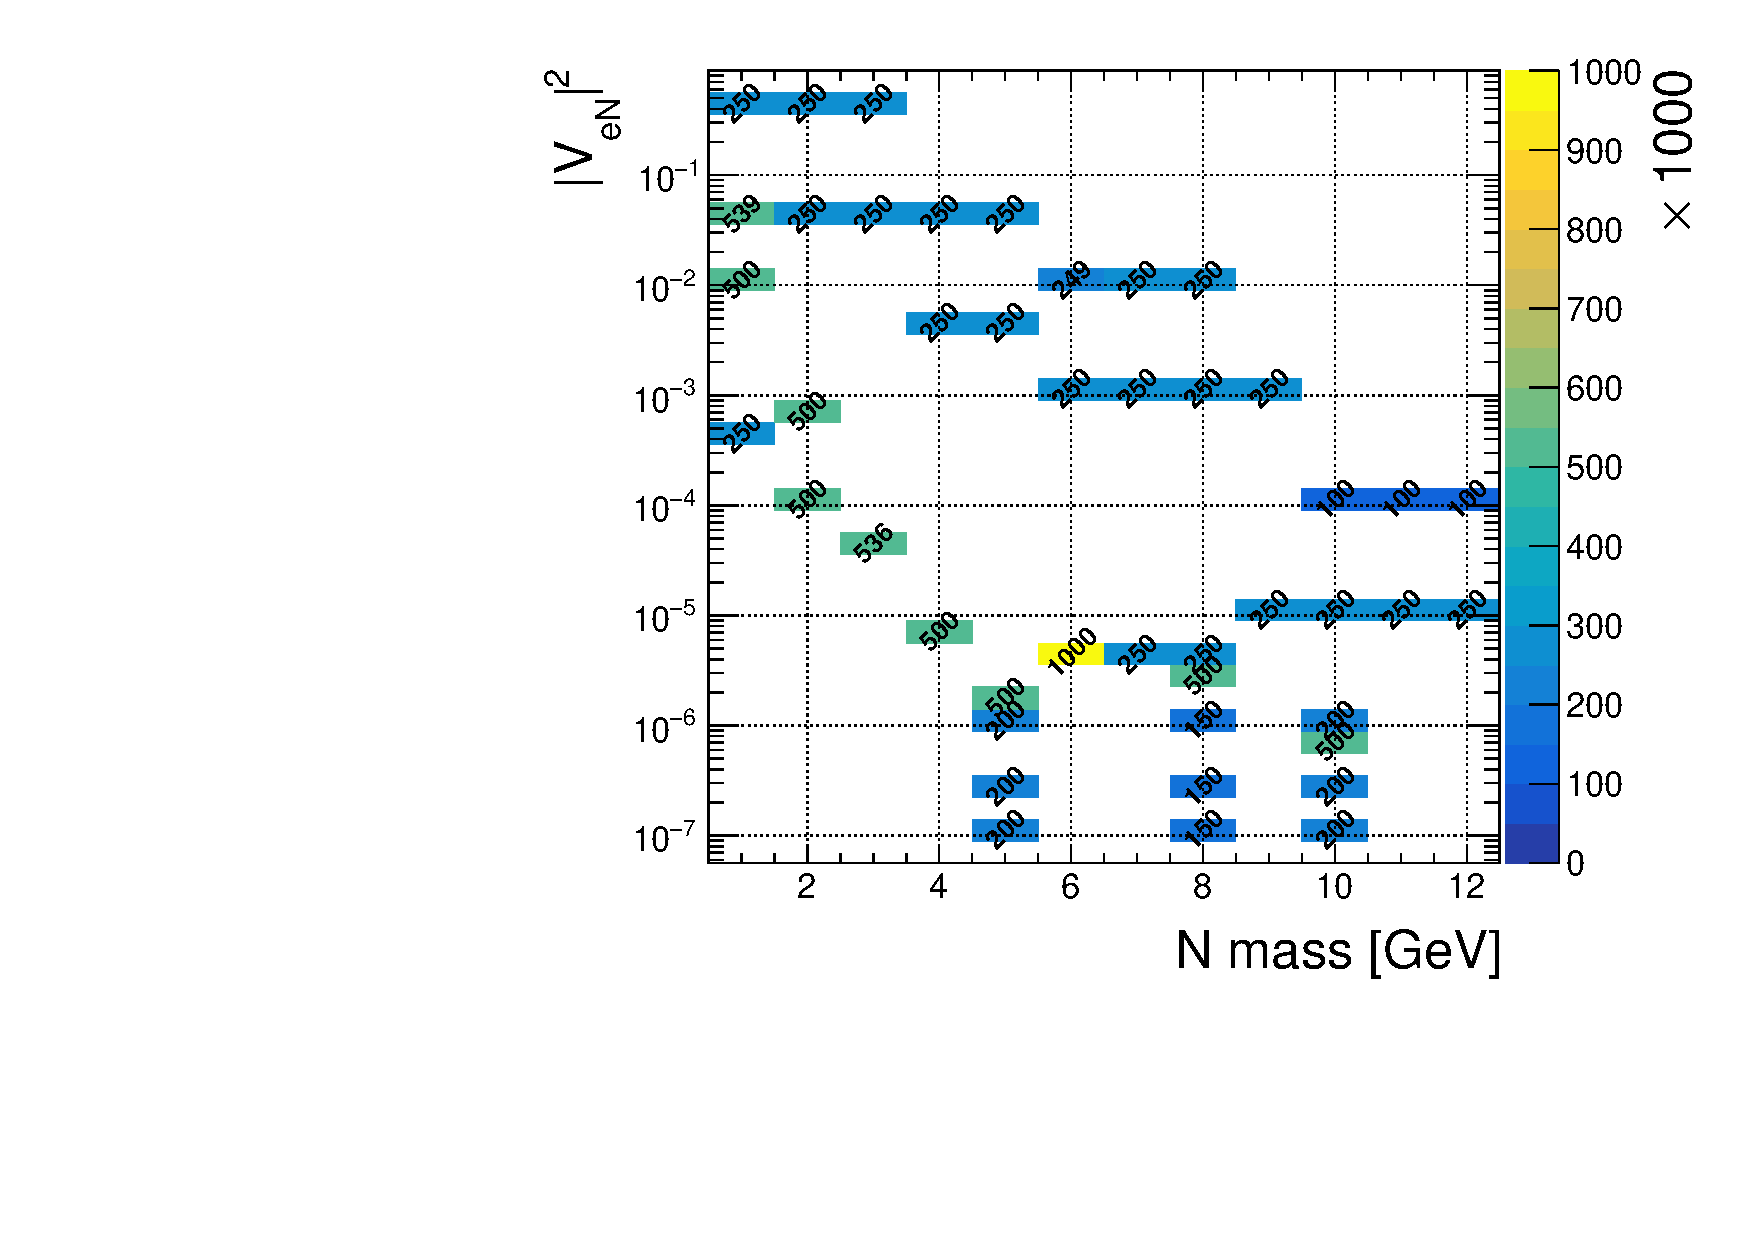
\includegraphics[width=0.68\textwidth]{Figures/c4/ll_hnl_samples_e.pdf}\\
  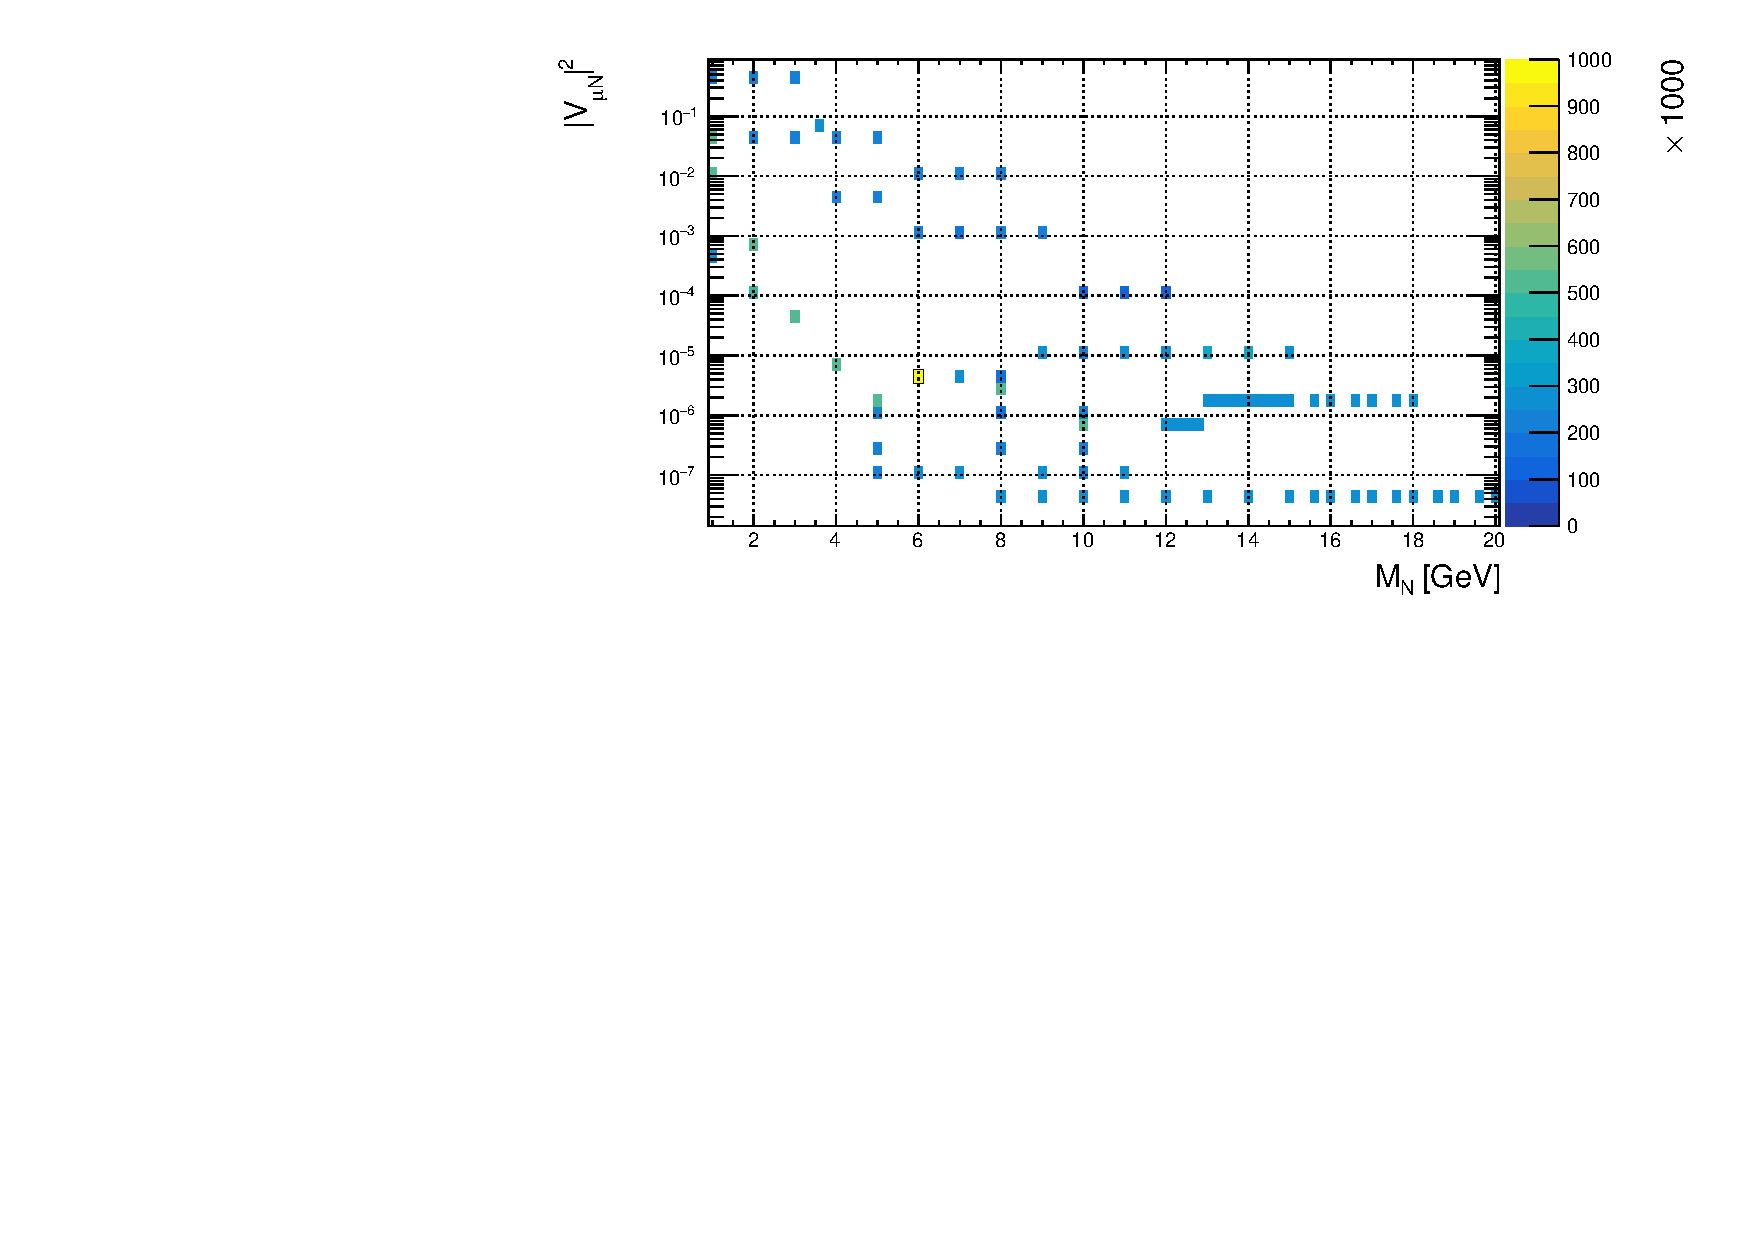
\includegraphics[width=0.68\textwidth]{Figures/c4/ll_hnl_samples_mu.pdf}
  \caption{Total number of signal MC events available for each
    $(\mhnl,\mixpar)$ point, considering both private and central CMS
    productions, for the electron (top) and muon (bottom) mixing
    parameters.}
  \label{fig:hnlSamples}
\end{figure}


\clearpage
